\subsection{Embodied Interaction}
While tool use is an important aspect of interactivity, most interaction in the real world does not happen through APIs. For example, humans are able to use natural language to communicate with other agents, to explore and manipulate their environment, and to learn from the consequences of their actions. Such embodied interaction requires an agent to understand the context, the goals, the actions, and the outcomes of each turn of interaction, and to adapt accordingly.
While \DV\ is obviously not embodied,  we explore whether it can engage in embodied interaction by using natural language as a text interface to various simulated or real-world environments. 


\subsubsection{Warmup: navigating a map}
In Figure~\ref{fig:mapz}, we prepare a ``map'' of a house, and ask \DV to explore it through interactive queries.
We then ask it to describe it in language and in a visualization, and compare that to the true map.
While it does not explore the whole house, \DV\ accurately describes what it does explore, even though all of its interactions are through this restricted text interface.

\begin{figure}[h!]
\begin{AIbox}{\DV}
%\begin{tcolorbox}[top=10pt, colback=white, colframe=black, colbacktitle=black, center, enhanced, breakable,
%attach boxed title to top left={yshift=-0.1in,xshift=0.15in},
%boxed title style={boxrule=0pt,colframe=white,}, title=\DV]
\parbox[t]{0.25\linewidth}{\tiny\begin{alltt} Human: You want to navigate through the map to reach the goal room. You start in the main room. Each round, you can choose to move left, right, up, down.
\\
Human: You are at the main room.
\\
AI: \hl{move left}
\\
Human: You enter kitchen 1. 
\\
AI: \hl{move up}
\\
Human: There is no way there.
\\
AI: \hl{move right}
\\
Human: You enter the main room.
\\
AI: \hl{move down}
\\
Human: There is no way there. 
\\
AI: \hl{move left}
\\
Human: You enter kitchen 1.
\\
AI: \hl{move right}
\\
Human: You enter the main room.
\\
AI: \hl{move up}
\\
Human: There is no way there.
\\
AI: \hl{move right}
\\
Human: You enter lobby.
\\
AI: \hl{move right}
\\
$\cdots$
\\
$\cdots$
\\
AI: \hl{move up}
\\
Human: You enter the room 1.
\\
AI: \hl{move right}
\\
Human: You enter the goal room!
\\
\end{alltt}} %
\parbox[t]{0.75\linewidth}{\tiny\begin{alltt} 
Human: Can you describe the locations of those rooms/halls etc?

AI: \hl{Sure, I can try to describe the locations of those rooms/halls etc. based on the map.

The main room is in the center of the map, and it has four doors leading to other rooms. The door on the left leads to kitchen 1, which is a small room with a stove, a sink, and some cabinets. The door on the right leads to the lobby, which is a large room with a sofa, a table, and some paintings. The door on the top leads to a dead end, and the door on the bottom leads to another dead end.

The lobby has three doors. The door on the left leads to the main room, the door on the bottom leads to the garden, and the door on the top leads to the hall 1. The garden is a green area with some flowers, trees, and a fountain. The hall 1 is a long corridor with some windows and doors on both sides.

The garden has two doors. The door on the top leads to the lobby, and the door on the right leads to the forest 1. The forest 1 is a dark and dense area with some bushes, rocks, and animals. The forest 1 has no other doors.

The hall 1 has four doors. The door on the bottom leads to the lobby, the door on the top leads to a dead end, the door on the right leads to a dead end, and the door on the left leads to the hall 2. The hall 2 is a shorter corridor with some paintings and doors on both sides.

The hall 2 has three doors. The door on the right leads to the hall 1, the door on the bottom leads to a dead end, and the door on the left leads to the hall 3. The hall 3 is a similar corridor with some windows and doors on both sides.

The hall 3 has three doors. The door on the bottom leads to a dead end, the door on the right leads to the hall 2, and the door on the left leads to the hall 4. The hall 4 is a narrower corridor with some lamps and doors on both sides.

The hall 4 has three doors. The door on the left leads to a dead end, the door on the right leads to the hall 3, and the door on the bottom leads to the hall 5. The hall 5 is a wider corridor with some rugs and doors on both sides.

The hall 5 has four doors. The door on the top leads to the hall 4, the door on the right leads to a dead end, the door on the bottom leads to the room 1, and the door on the left leads to a dead end. The room 1 is a cozy room with a bed, a desk, and a closet.

The room 1 has two doors. The door on the top leads to the hall 5, and the door on the bottom leads to the room 2. The room 2 is a similar room with a bed, a desk, and a closet.

The room 2 has one door. The door on the top leads to the room 1.

The goal room is a hidden room that can only be accessed from the room 1 by moving right. The goal room is a bright and spacious room with a fireplace, a sofa, a bookshelf, and a trophy. The goal room has no other doors.}
\end{alltt}}
\\
{\DV} summarizing what it ``sees'' after it navigates through the map. The number of doors in each room in {\DV}'s summary is exactly equal to the number of directions {\DV} tried in each room. {\DV} also ``imagines'' what the rooms look like simply based on their names and connections.
\\
\parbox[t]{\linewidth}{\tiny\begin{alltt}
Human: Can you draw a pyplot plot showing the position of the rooms/places and connect them using lines? \end{alltt}}
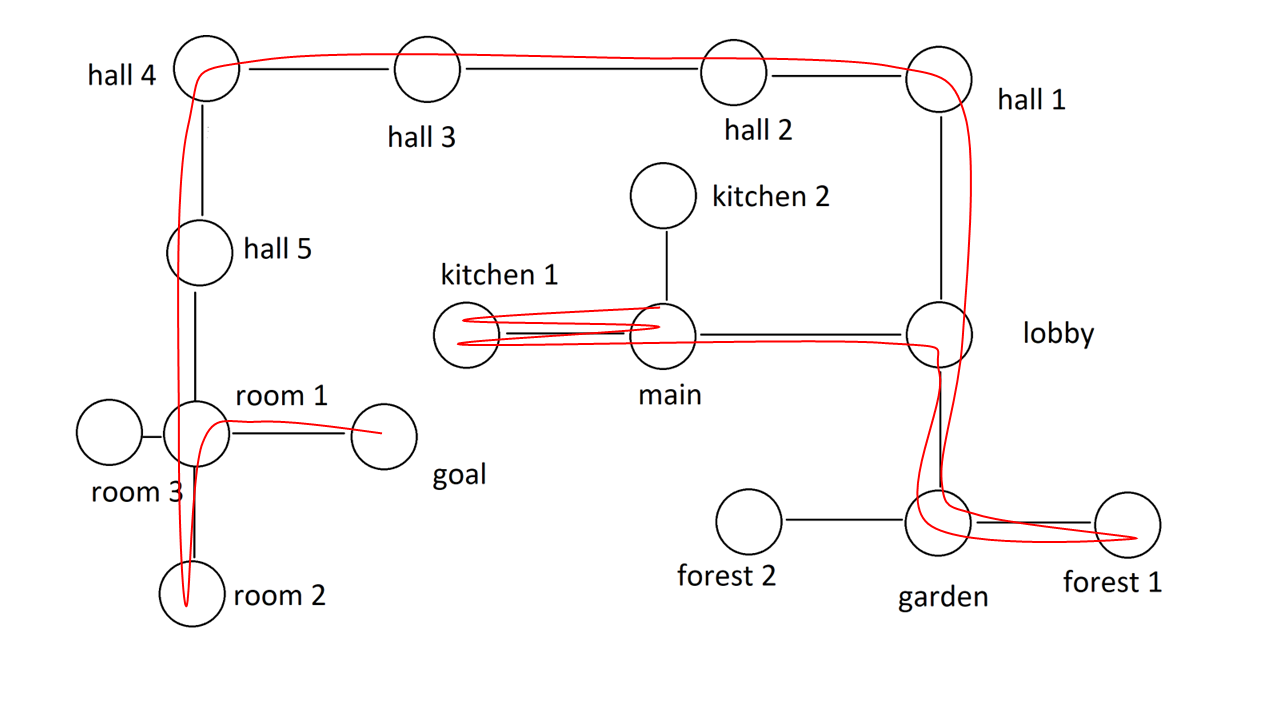
\includegraphics[width=0.45\linewidth]{figures/room_path_dv3.png} \hfill 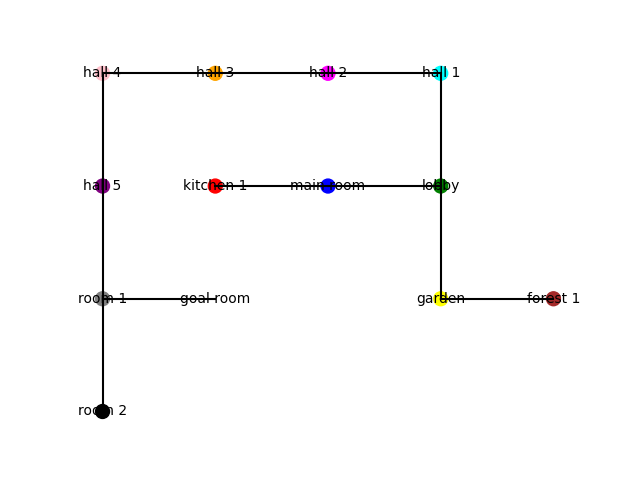
\includegraphics[width=0.45\linewidth]{figures/room_dv3.png}
\\
Left: The true map and exploration path of {\DV}. Right: The map that {\DV} generates. We see that {\DV} accurately tracks all the locations of the room from the exploration and visualized them correctly.

\end{AIbox}
\caption{\DV\ navigates a map interactively, then describes it in different modalities}
\label{fig:mapz}
\end{figure}

\subsubsection{Text-based games}
\label{sec:game1}

Text-based games are a natural and challenging domain for language models, as they require understanding natural language, reasoning about the game state, and generating valid commands. A text-based game is a type of interactive fiction, where an agent interacts with an environment through natural language descriptions and commands. The agent has to perform a given task, such as finding a treasure or escaping a dungeon, by exploring the environment and manipulating objects. We first test if \DV\ can explore the environment in text-based games to perform the given task. In this and the next experiments, we use TextWorld~\cite{cote2018textworld}, a framework for generating and playing text-based games, to create two games with different given tasks.

\paragraph{Exploring the environment.}
The first game takes place in a house with many rooms, and the objective is to find and unlock a certain chest by navigating between different rooms.
This game is relatively simple, as it does not involve any inventory management, crafting, or combat.
The environment is described by a text paragraph, and the player can type commands such as ``go north'', ``examine couch'', or ``open chest''.
The chest is usually few rooms away from the starting point, and thus solving the game requires exploring the environment without getting lost.

We give the exact initial text from Textworld as the initial prompt, and issue \texttt{help} as a first command. After that, \DV\ plays the game as a normal player. It completes the game in 30 actions without any extra help, and navigates the environment efficiently without looping through rooms (Fig.~\ref{fig:game1} contains an excerpt and the route taken, and Appendix~\ref{sec:game1_log} has the complete log). Qualitatively, \DV\ solves the game in a very conservative manner, by examining and picking up every object in each room regardless of its relevance to the game objective. In contrast, however, \texttt{text-davinci-003} does not respond to the environment feedback at all, issuing the same command repeatedly (Appendix~\ref{sec:game1_log_chatgpt}).

\begin{figure}[t] % h means place the figure here if possible
\centering % center the figure
\parbox{0.55\textwidth}{
\begin{AIbox}[width=0.55\textwidth]{\DV}\scriptsize
\begin{alltt}
> \hl{take Canadian latchkey}\\
You pick up the Canadian latchkey from the ground.\\
> \hl{unlock Canadian chest with Canadian latchkey}\\
You unlock the Canadian chest.\\
Your score has just gone up by one point.\\
*** The End ***
\end{alltt}
\end{AIbox}}
\raisebox{-0.5\height}{
\resizebox{6cm}{4cm}{
\begin{tikzpicture}[node distance=1cm, every node/.style={draw, minimum width=2cm, minimum height=1cm}]
\node (attic) {Attic};
\node (spare) [right=of attic] {Spare Room};
\node (cellar) [right=of spare] {Cellar};
\node (bedchamber) [above=of attic] {Bedchamber};
\node (cookhouse) [right=of bedchamber] {Cookhouse};
\node (scullery) [right=of cookhouse] {Scullery};
\node (bedroom) [above=of cookhouse] {Bedroom};

% route by the player
\draw[->] (attic) to[bend right=15] node[below, draw=none, yshift=0.25cm] {1} (spare);
\draw[->] (spare) to[bend right=15] node[above, draw=none, yshift=-0.25cm] {2} (attic);
\draw[->] (attic) -- node[left, draw=none, xshift=0.8cm] {3} (bedchamber);
\draw[->] (bedchamber) -- node[above, draw=none, yshift=-0.25cm] {4} (cookhouse);
\draw[->] (cookhouse) -- node[below, draw=none, yshift=0.25cm] {5} (scullery);
\draw[->] (scullery) to[bend right=30] node[above, draw=none, yshift=-0.25cm] {6} (cookhouse);
\draw[->] (cookhouse) to[bend left=30] node[right, draw=none, xshift=-0.8cm] {7} (spare);
\draw[->] (spare) -- node[below, draw=none, yshift=0.25cm] {8} (cellar);
\draw[->] (cellar) to[bend right=30] node[above, draw=none, yshift=-0.25cm] {9} (spare);
\draw[->] (spare) to[bend left=30] node[left, draw=none, xshift=0.7cm] {10} (cookhouse);
\draw[->] (cookhouse) -- node[left, draw=none, xshift=0.7cm] {11} (bedroom);
\end{tikzpicture}}}
\caption{The left figure shows the last two commands from \DV\ and the environment response for the first game in Section~\ref{sec:game1}. The right figure shows the route \DV\ takes.}
\label{fig:game1}
\end{figure}


\paragraph{Responding to feedback.}
\label{sec:game2}

Here \DV\ plays a game where the task is to prepare a two-ingredient, five-step meal according to a cookbook. This game is more challenging than the previous one because the player (\DV) has to figure out key commands by itself from the environment response (these are not listed in \texttt{help}), such as cutting the food, using the right utensils, and turning on the appliances (see Fig.~\ref{fig:game2}). 

\DV\ uses trial and error when playing the game, but it also adapts to the environment and generalizes between actions. For example, it learns that the \texttt{chop} command requires a knife in Fig.~\ref{fig:game2},  and it does not make the same mistake afterward. It follows the instructions from the cookbook, but also infers some missing actions such as taking the required ingredients.
While the game does not specify that key commands are missing, \DV\ makes reasonable guesses, e.g., when it fails to grab a frying pan from the kitchen, it goes into a bedroom to \texttt{look for a frying pan} (more details in Appendix~\ref{sec:game2_log}).
\DV\ cannot solve this game, but neither could the authors of this paper (who got stuck in the same step) prior to looking at the source code.
However, if we give \DV\ a one-shot demonstration of creating a different meal, it is able to generalize from it and solve the game (Appendix~\ref{sec:game2_log_shot1}). 

% To further test \DV's ability to learn from feedback, we give it a demo (including the commands and outcomes) for preparing a different meal as the prompt to \DV. This demo involves a key step for the task ``roast the lettuce'' (\texttt{cook lettuce with oven}). We then ask it to cook the original meal involving the apple it could not solve before. We observe that \DV\ can generalize from the demonstration and apply a similar step to fry the apple (\texttt{cook apple with stove}). See Section~\ref{sec:game2_log_shot1} for the details.



\begin{figure}[t] % h means place the figure here if possible
\centering % center the figure
\begin{AIbox}[width=0.6\textwidth]{\DV}
\scriptsize \begin{alltt}
> \hl{chop the red hot pepper}
Cutting something requires a knife.
> \hl{chop the red hot pepper with the knife}
You need to take the red hot pepper first.
> \hl{take the red hot pepper}
You take the red hot pepper from the counter.
> \hl{chop the red hot pepper with the knife}
\end{alltt}
\end{AIbox}
\caption{Examples of \DV\ reacting to the environment in the second game in Section~\ref{sec:game2}}
\label{fig:game2}
\end{figure}

\subsubsection{Real world problems}   
In Fig.~\ref{fig:human_affordance} and Fig.~\ref{fig:human_affordance2}, \DV\ is given two real-world problems to solve, and given \emph{a human} as a partner (i.e., a very flexible agent with very little constraints, who can also respond in natural language) to interact with the environment.
Both problems were real problems faced by authors of this paper, who responded to \DV\ in such a way as to track the situation they faced. For both problems, \DV\ is able to identify the actions the human needs to take in order to address the problem. In the first example, \DV\ guides the human to find and fix a water leak and recommends the exact actions that the human took (after replacing the seal, the leak was gone).
% TODO: This is in appendix, so probably should not refernece
In the second example, the author had not called the gas company to transfer service from the old user, and thus the gas was turned off.
In this case, \DV\ is able to quickly arrive at the source of the problem (the actual human took a long time to check the pilot light in the water heater), and propose plausible solutions. However, it is not able to diagnose the root cause until the human himself has the idea to check the stove-top.

\subsubsection{Discussion}
While it is clearly not embodied, the examples above illustrate that language is a powerful interface, allowing \DV\ to perform tasks that require understanding the environment, the task, the actions, and the feedback, and adapting accordingly.
While it cannot actually see or perform actions, it can do so via a surrogate (e.g., a human).
Having said this, we acknowledge the limitation that we only tested \DV\ on a limited number of games and real-world problems, and thus cannot draw general conclusions about its performance on different types of environments or tasks. A more systematic evaluation would require a larger and more diverse set of real world problems where \DV\ was actually used in real-time, rather than retrospectively.

% TODO
% This latter case in particular illustrates situations where new tools are brought in as the situation evolves -- for example, the suggestion of calling a plumber in Fig.~\ref{fig:human_affordance} or calling a professional in Fig.~\ref{fig:human_affordance2} after other options were exhausted.

\begin{figure}
\begin{AIbox}{\DV}
\parbox{1\textwidth}{\scriptsize\begin{alltt} \vspace{-6px}
The computer is trying to solve a problem. It can tell the human to do anything, one thing at a time, and one line at a time.

PROBLEM: there is water dripping from the kitchen ceiling, and you have to figure out why and fix it

----<|endofprompt|>

Human: The kitchen ceiling is dripping water

\hl{Computer: Check to see if there is a bathroom or other water source directly above the kitchen.}\\

Human: Yes, there is a bathroom actually

\hl{Computer: Check the bathroom for any signs of water leakage, such as puddles on the floor, water dripping from the ceiling, or water stains on the walls.}\\

Human: There is a little water on the floor

\hl{Computer: Try to identify where the water is coming from. Check the toilet, sink, and bathtub/shower for any leaks.}\\

Human: It is next to the bathtub and the toilet

\hl{Computer: Check the seals around the bathtub and toilet to see if they are worn or damaged. If they are, replace them. If they are not, continue investigating other potential sources of the leak.
}\\

Human: I can't see the seal around the toilet, there is a porcelain thing around it. I don't see any damage in the bathtub seal though

\hl{Computer: If you can't see the seal around the toilet, you may need to remove the porcelain cover to inspect it. If you don't feel comfortable doing this, you may need to call a plumber.}\\

Human: Ok, I removed it. But I can't tell if it's damaged or not

\hl{Computer: If you can't tell, it may be best to replace the seal anyway, just to be sure. If the leak persists after replacing the seal, you will need to continue investigating other potential sources of the leak.
}\end{alltt}}\vspace{-6px}
\end{AIbox}
\caption{\DV\ acts as a virtual handyman.}\label{fig:human_affordance}
\end{figure}
